\subsection*{Line-Of-Sight Propagation}
\paragraph{Introduction}
At low frequency (below approximately 3 MHz) radio signals travel as ground waves, which follow the Earth's curvature due to diffraction with the layers of the atmosphere.
However, at higher frequencies and in lower levels of the atmosphere, neither of these effects are significant. Thus any obstruction between the transmitting antenna (transmitter) and the receiving antenna (receiver) will block the signal, just like the light that the eye may sense. Therefore, since the ability to visually see a transmitting antenna (disregarding the limitations of the eye's resolution) roughly corresponds to the ability to receive a radio signal from it, the propagation characteristic of VHF and higher radio frequency (>30 MHz) paths is called line-of-sight. The farthest possible point of propagation is referred to as the radio horizon.\\

The radio horizon is the locus of points at which direct rays from an antenna are tangential to the surface of the Earth. If the Earth were a perfect sphere and there were no atmosphere, the radio horizon would be a circle.
This way the greatest distance at which a receiver can see the transmitter is explained in the following paragraph.

\paragraph{Geometrical model}

First, we are going to derive a general expression and after that apply it to a scenario with a drone and a basestation. In figure  \ref{fig:GeometricDist_general} the relationship between the height of the observer above sea level (O point) and the distance d which is between it and the horizon (H point) is shown. Finding this distance is done by the use of the pythagorean theorem. With some simple mathematical calculations the distance d is derived in the following:
\begin{align}
&(R+h)^2 = R^2+d^2\nonumber \\
&\Rightarrow R^2+2hR+h^2 = R^2+d^2 \Rightarrow d^2 = 2hR + h^2 \\
&\Rightarrow d = \sqrt{2hR + h^2} \label{eq:los_distToHorizon}
\end{align}

\begin{figure}%
    \centering
    \subfloat[Geometrical distance to the horizon]{{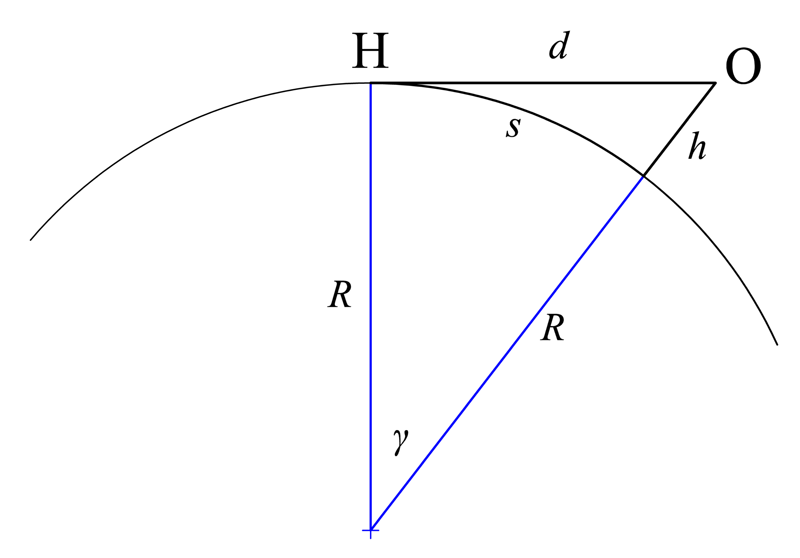
\includegraphics[width=6cm]{figures/GeometricDistanceToHorizonOneTriangle.png} 
\label{fig:GeometricDist_general}   }}%
    \qquad
    \subfloat[Geometrical distance from drone to basestation]{{
    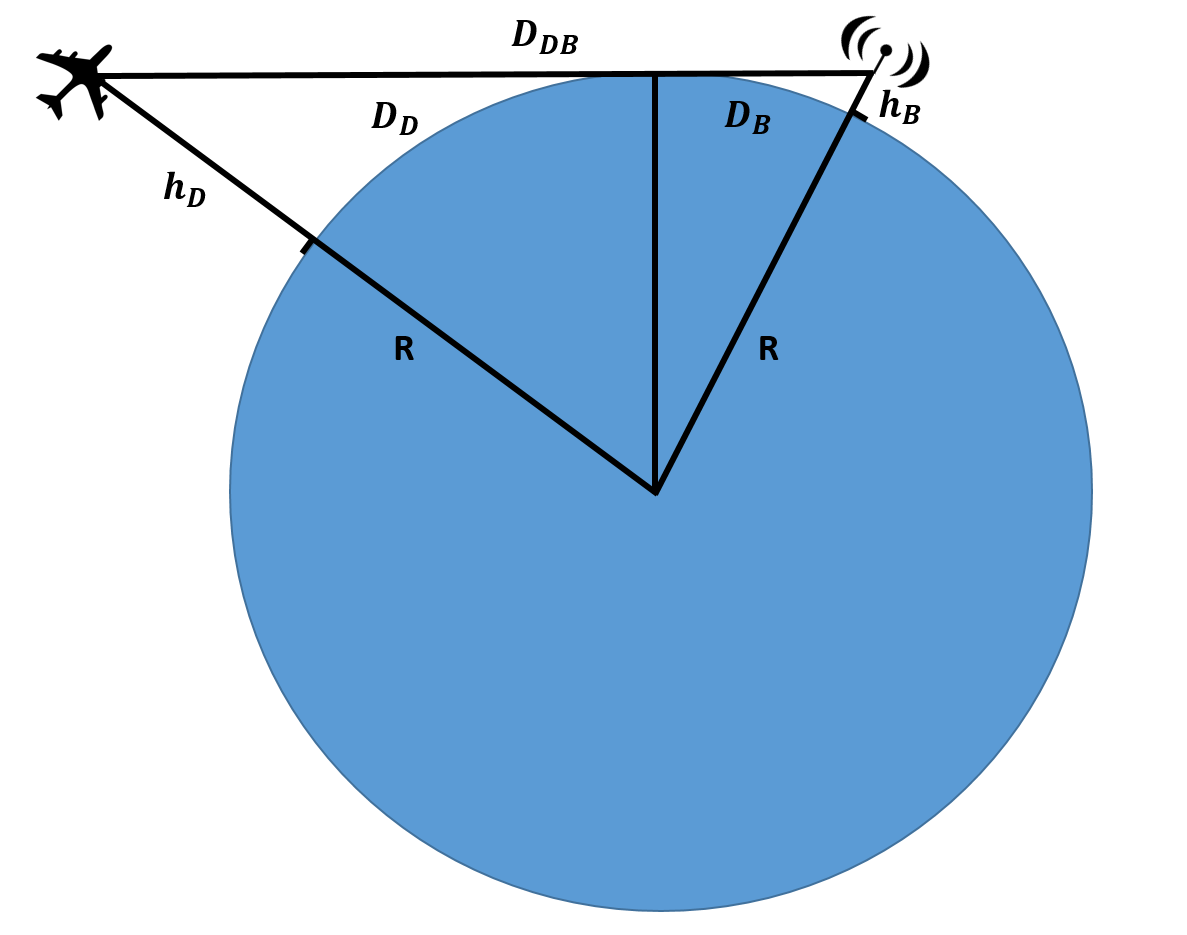
\includegraphics[width=6cm]{figures/GeometricDistanceToHorizonTwoTriangle.png} 
    \label{fig:GeometricDist_droneBasestation}  }}%
    \caption{Geometrical distance to the horizon, Pythahorean theorem}%
    \label{fig:GeometricDistanceToHorizon}%
\end{figure}

On figure \ref{fig:GeometricDist_droneBasestation} it is shown that the two objects are a drone and a basestation. Both of them wont be higher then approx 100 meter and since R is radius of the Earth, $2hR$ >> $h^2$ and $h^2$ is therefore neglected in equation \ref{eq:los_distToHorizon}. The two distances $D_D$ and $D_B$ have the same expressions in both cases:
\begin{align}
D_D [km] &= \sqrt{2\cdot R \cdot h_D + h_{D}^2} \approx \sqrt{2\cdot 6.378\cdot h_D} = \sqrt{12.756\cdot h_D} = 3.57\cdot \sqrt{h_D} \\
D_B [km] &= \sqrt{2\cdot R \cdot h_B + h_{B}^2} \approx \sqrt{2\cdot 6.378\cdot h_B} = \sqrt{12.756\cdot h_B} = 3.57\cdot \sqrt{h_B}
\end{align}
To calculate the distance $D_{DB}$:
\begin{align}
D_{DB}[km] &= D_D + D_B \approx 3.57\cdot \sqrt{h_D} + 3.57\cdot \sqrt{h_B} = \underline{3.57\cdot (\sqrt{h_D} + \sqrt{h_B}} )
\end{align}

\subsection{Example with drone = 100m and basestation = 20m}
Lets take an example if the drone is at $h_D = 100m$ and the basestation at $h_B = 20m$. The distance between the drone and the basestation is as follows:
\begin{align}
D_{DB}[km] = 3.57\cdot (\sqrt{100} + \sqrt{20}) = 51.67km
\end{align}
